\subsection{Integrazione tra Arena ed interfaccia grafica}
Durante il primo sprint abbiamo lavorato a stretto contatto dato che uno si occupava della creazione dell'interfaccia grafica e l'altro della creazione dell'arena di gioco a livello logico.

Il grosso problema da risolvere era quello di mappare la posizione logica delle varie entità all'interno di un'interfaccia grafica.
Dopo varie proposte si è arrivati alla soluzione attuale: dare ad ogni difficoltà una grandezza logica [\ref{difficulty}] dell'arena di gioco per poi andare a suddividere la finestra grafica in piastrelle (Tile) di dimensione pari al rapporto tra la grandezza della finestra fisica e quella logica [\ref{tile}].

Così facendo si può facilmente mappare un punto logico (\textit{Point}) in un pixel [\ref{conversion}].

\begin{figure}[H]
    \centering
      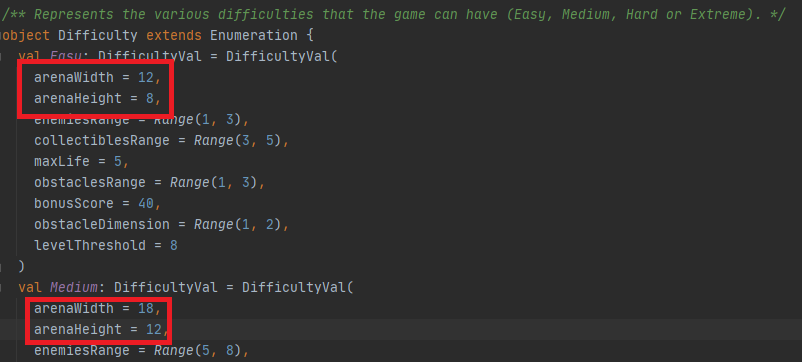
\includegraphics[width=13cm]{res/6-implementazione/chianapasini/difficulty.png}
      \caption{Dimensione logica delle difficoltà}
      \label{difficulty}
    \end{figure}
    
\begin{figure}[H]
    \centering
      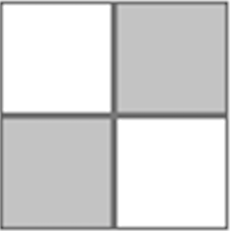
\includegraphics[width=13cm]{res/6-implementazione/chianapasini/tile.png}
      \caption{Dimensione tile}
      \label{tile}
    \end{figure}
    
\begin{figure}[H]
    \centering
      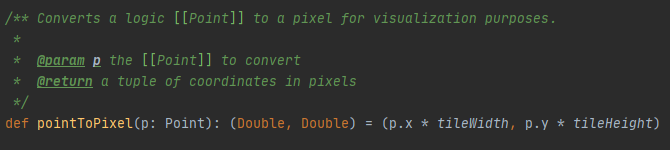
\includegraphics[width=13cm]{res/6-implementazione/chianapasini/conversion.png}
      \caption{Mappatura tra Point e pixel}
      \label{conversion}
    \end{figure}